\documentclass{article}                     % onecolumn (standard format)

\usepackage{graphicx}
\usepackage{float}
\usepackage{amsmath}
\usepackage{cite}
\usepackage{subcaption}
\usepackage{rotating}
\usepackage[left=2.2cm, right=2.2cm]{geometry}
\usepackage{algpseudocode}
\usepackage{algorithm}
%\floatstyle{ruled}
\usepackage[hidelinks]{hyperref}
\usepackage{algpseudocode}
\usepackage{tikz}
\usetikzlibrary{positioning,calc,shapes,shapes.geometric}
\usepackage{pgf}
\usepackage{verbatim}

\newfloat{algorithm}{tbp}{loa}
\providecommand{\algorithmname}{Algorithm}
\floatname{algorithm}{\protect\algorithmname}


%\renewcommand{\thesection}{\Roman{section}}
\usepackage{titlesec}
\titleformat{\section}
{\normalfont\Large\bfseries}{Exercise~\thesection}{1em}{}



\newcommand{\relation}[3][]
{
	% this needed to be modified somehow...
	\path [draw=blue, ->,#1] (#2) -- (#3);
}

\newcommand{\mynode}[3][]{
	\node [draw, circle] (#1) at (#2, #3) {#1};
}
%\newcommand{newnode}[3]{
%\node[draw,fill=green,circle,label=north:#1] (#1) at (#2,#3) {};
%}


\begin{document}
	
	\title{Introduction to AI - assignment 6}
	
	
	\author{Oded~Yechiel}
	
	\date{8/1/19}
	
	\maketitle
	\tableofcontents
	\section{}
	\begin{verbatim}
	I({A,B},{C,D}|{})
	I({A,B},{C,D,G,H}|{})
	I({E,F},{C,D,G,H}|{})
	I({G},{C}|{D})
	
	not I({A},{B}|{})
	not I({C},{G}|{})
	not I({E},{F}|{})
	not I({C},{G}|{D,H})
	\end{verbatim}
	\subsection{Construct a Bayes network that is consistent with the  above set of independence statements}
	Since A and B are closed and are independent from all other nodes, they can be separated from the rest of the tree and just connected between themselves (since they are dependent). 
	
	Same goes for nodes E and F.
	
	Since C and G and dependent unless D is in evidence this suggests that D is a parent of both C and G. In addition, since C and G are dependent in the presence of H this suggests that C and G are parents of H.
	
	Fig.~\ref{fig:bn1} proposes a Bayes Network tree that supports all of the statements in the requirements.
	
	\begin{figure}
		\centering
		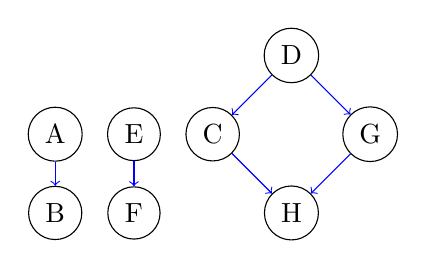
\begin{tikzpicture}
		\mynode[A]{0}{1}
		\mynode[B]{0}{0}
		\mynode[E]{1}{1}
		\mynode[F]{1}{0}
		\mynode[C]{2}{1}
		\mynode[D]{3}{2}
		\mynode[G]{4}{1}
		\mynode[H]{3}{0}
		%	\node [draw] (A) at (0, 0) {A};
		%	\node [draw] (B) at (3, 0) {B};
		%	\node [draw] (C) at (3, 3) {C};
		\relation{A}{B}
		\relation{E}{F}
		\relation{D}{G}
		\relation{D}{C}
		\relation{G}{H}
		\relation{C}{H}
		\end{tikzpicture}
		\caption{Bayesian Network}
		\label{fig:bn1}
	\end{figure}
	
	\subsection{Is the answer above unique?}
	\textbf{No}. As mentioned above H has to be the child of C and G, and D has to be their parents. However, A can be the parent of B, or B can be the parent of A. Same goes for E and F. Thus, there are $ 2^2 $ combinations, which add up to \textbf{4 possible BN that will hold the statements}.
	
	\section{}
	\begin{figure}
		\centering
		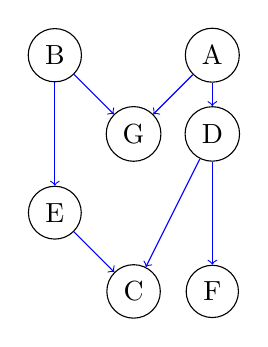
\begin{tikzpicture}
		\mynode[A]{3}{3}
		\mynode[B]{1}{3}
		\mynode[E]{1}{1}
		\mynode[F]{3}{0}
		\mynode[C]{2}{0}
		\mynode[D]{3}{2}
		\mynode[G]{2}{2}

		\relation{A}{D}
		\relation{A}{G}
		\relation{B}{G}
		\relation{B}{E}
		\relation{D}{C}
		\relation{E}{C}
		\relation{D}{F}
		\end{tikzpicture}
		\caption{Network tree}
		\label{fig:bn2}
	\end{figure}
	\subsection{Is this network a poly-tree?}
	\subsection{Is this network (directed-path) singly connected?}
	\subsection{Determine the truth of the following independence statements (using d-separation)}
	\begin{enumerate}		
		\item \begin{verbatim} I({D}, {E} | {    }) - False \end{verbatim}
		\item \begin{verbatim} I({D}, {E} | {  A }) - True \end{verbatim}
		\item \begin{verbatim} I({D}, {E} | {A, C}) - False \end{verbatim}
		\item \begin{verbatim} I({B}, {F} | {  G }) - True \end{verbatim}
		\item \begin{verbatim} I({B}, {F} | {  D }) - True \end{verbatim}
		\item \begin{verbatim} I({B}, {F} | {A, C}) - False \end{verbatim}

	\end{enumerate}

	\subsection{Find P(E=true, A=True $ | $ B=true)}
	\begin{verbatim}
	P(A=true) = 0.2, P(B=true)= 0.3
	P(G=true|A=true,B=true) = 0.9, P(G=true|A=false,B=true) = 0.2
	P(G=true|A=true,B=false) = 0.5, P(G=true|A=false,B=false) = 0.1
	P(E=true|B=true) = 0.8, P(E=true|B=false) = 0.1
	P(C=true|D=true, E=true) = 0
	\end{verbatim}
	
	Since G and C are not in evidence and B is in evidence, we can safely say that A and E are statistically independent. Moreover, A and B are also independent since G and C are not in evidence. Hence
	
	$ P(E, A | B) =P(E|B)*P(A|B)=P(E|B)*P(A)=0.8 * 0.2 = 0.16 $
	
	
	\section{}
	\subsection{Can this be done without hidden units?}
	\textbf{No.} It is impossible with no hidden layers to predict a non-linear function such as modulu. However, for this simple example, a single hidden layer will suffice as shown in the following subsection.
	
	\subsection{Show a network using threshold elements that performs the required computation}
	We will use a neural network with 1 hidden layers that is composed of 6 neurons. This means for the input layer (6 neurons), the hidden layer will have 36 weights (6 x 6 matrix - M1) and 6 bias weights that are summed and enter a $ tanh $ activation function. 
	
	The output, a 6x1 vector $ X1 $ is then bitwise multiplied by 6 weights (one for each neuron) summed and are added with the bias $ b2 $. The output is passed through a sigmoid activation function and the result is rounded to decide if the result is '0' or '1'.
	
	The complete code in Keras that generates the dataset and labels, trains, and provides the weights can be found, along with this report, in the git repository at 
	\begin{equation}\label{eq:m1}
	M1 = \left[ \begin{array}{cccccc}
		-2.6035163 & 1.0730004 & 0.73517716 &  0.7892835 & 2.0436563 & -3.0340612 \\
		-2.8252845 & 1.1691521 & 1.3764652 & 1.5624126 & -3.209769 &	-2.571492  \\
		-2.5988533 & 1.1376183 & 0.9316116 & 0.563356  & 2.0437527 & -3.031866  \\
		-2.5722306 & 1.2495581 & 0.7956654 & 0.7881598 & 2.0363252 &	-3.0355027 \\
		-2.603346  & 1.1103705 & 0.60637933 & 0.61684054 & 2.0353322 & -3.025518 \\
		-2.5890596 & 1.0401373 & 0.26387808 & 1.0831383 & 2.0149522 &  -3.0376844 \\
	\end{array} \right]
	\end{equation}
	\begin{equation}\label{eq:b1}
	b1 = \left[8.979317  , -5.988329  ,  0.26482144, -0.250453  , -1.1340998 ,
	6.665368 \right]^T
	\end{equation}
	\begin{equation}\label{eq:m2}
	M2 = \left[\begin{array}{c}
	6.996323 \\
	  4.3360047\\
	 -0.807298\\
	 -0.6610357\\
	 -1.4745305\\
	-10.0931015
	\end{array}\right]
	\end{equation}
	\begin{equation}\label{eq:b2}
	b2 = -2.8664327
	\end{equation}
	\begin{equation}\label{eq:l1}
	X1 = tanh(M1 \times X + b1)
	\end{equation}
	\begin{equation}\label{eq:l2}
	\hat{y} = round(sigmoid(M2 \times X1) + b2)
	\end{equation}
\end{document}

